%!TEX root = shrink.tex
\section{Energy vs. user-perceived latency model}
\label{sec:analysis}

We present a simple analytical model in order to quantify the relationship between energy savings and user-perceived latency inflation in \cdc s, and to gain a deeper understanding of the factors that determine this trade-off. The primary purpose of this model is expository, so we make a number of simplifying assumptions for ease of exposition first, and we progressively relax them in this and subsequent sections.

%In this section, we present an analytical model of server consolidation which a goal of answering the following questions. (1) What are the system and workload characteristics required to achieve a good energy-performance tradeoff? (2) Can real systems and workloads be expected to satisfy those requirements? 

%For a qualitative understanding of the factors that determine the goodness of the energy-latency tradeoff, we present an analytical model of server consolidation in \cdc s. We focus on a Zipf content workload the analyze the effect of the skewness of the Zipf workload and the server-load-dependent queuing latency on the energy-latency tradeoff.

\begin{figure}
\centering
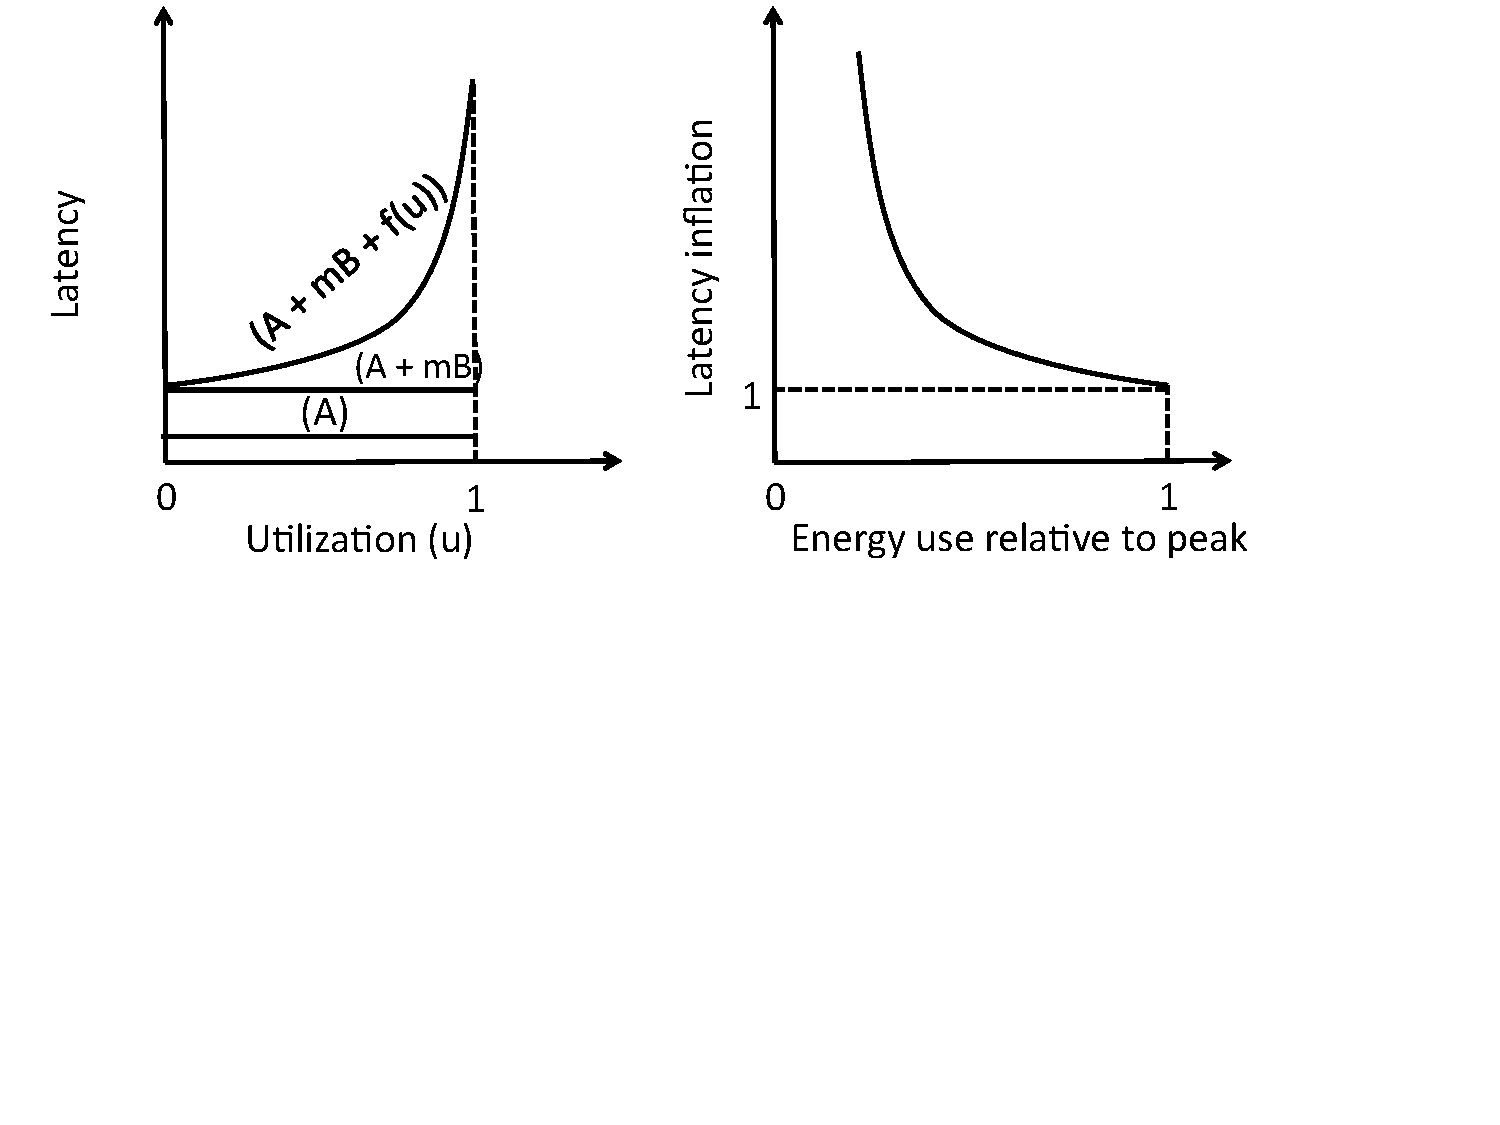
\includegraphics[scale=0.36]{figures/model.pdf}
\vspace{-1.5in}
\caption{[Left] An illustrative server utilization vs. latency curve. [Right] Corresponding energy-latency curve.}
\label{fig:model}
\end{figure}

\subsection{Single server}
\label{sec:singleserver}
Consider a single \cdc\ server serving a workload of content requests from end users that is unchanging, i.e., the arrival rate, popularity distribution, and size distribution of content across requests is fixed. Let $m$ denote the cache miss rate at the server, i.e., the fraction of requests for which the server contacts the origin server. Assume that the power drawn by a server $p(u)$ is a linear function of its utilization $u$, or the ratio of the incoming load and the server's capacity \cite{mathew12}. In this model, an idle server's power consumption is a fraction $I$ of its peak power $P$, and the power consumed increases linearly from $IP$ to $P$ as the utilization increases from 0 to 1, i.e., $p(u) = (I + (1-I)u)P$.

The end-to-end user-perceived latency is assumed to be the sum of three components as also illustrated by the three curves in Figure \ref{fig:model} (left): (1) Mean server latency $f(u)$, assumed to be a convex, increasing function of the utilization $u$ $(0\leq u\leq1)$; (2) Server-to-origin latency $B$, which is constant but incurred only upon a cache miss; (3) Client-to-server latency $A$, a constant. Thus, the total end-to-end user-perceived latency is $f(u) + mB + A$. As shown in the figure, realistic utilization vs. server latency profile are typically somewhere in between a straight line where the latency increases linearly with the utilization and an $L$-shaped curve where the latency is zero for all values of utilization less than 1 and is infinity at 1.

\subsection{Datacenter as a single logical server}
\label{sec:multiserver}

The simplistic model above can serve as a first-order approximation of a datacenter viewed as a single logical server as follows. Suppose the datacenter consists of $N$ homogeneous servers, each identical to the one above. Suppose the total incoming load is uniformly distributed across all $N$ servers resulting in a fixed utilization $U$ at each server, which implies a power consumption of $(I+(1-I)U)P$ per server. Thus, the total power consumed is $(I+(1-I)U)PN$, and the mean latency is $f(U) + mB + A$. We have implicitly assumed here that the miss rate $m$ remains the same as above even though each server is getting a sampled transformation of the original request distribution.

What is the impact of consolidating the datacenter to $n<N$ servers on the total power consumed and user-perceived latency? To answer the first part, we observe that the utilization at each server increases by a factor $N/n$, so its power consumption would increase to $(I+(1-I)UN/n)P$. Thus, the consolidated datacenter's total power consumption is given by $(nI + (1-I)UN)P$, and the corresponding energy use relative to the peak (the x-axis in Figure  \ref{fig:model} (right)) is 
\begin{eqnarray}
\textit{benefit}  = \frac{ (nI + (1-I)UN)P}{(I+(1-I)U)PN}
\label{eq:benefit}
\end{eqnarray}

Computing the corresponding end-to-end latency with the consolidation as above is nontrivial as it requires us to account also for the increase in cache miss rates. Assuming that shutting down servers results in a proportional decrease by a factor $N/n$ in the total available storage (an assumption that is natural for clusters of commodity PCs--the more common option in practice--but not for CDCs relying on network storage), we need to compute the mean miss rate $m'$ that in general would be lower than $m$. In our numerical examples below, we derive $m'$ using a characteristic-time approximation model for an LRU cache \cite{che2002hierarchical}. 
The latency is given by $f(UN/n) + m'B + A$, and the corresponding latency 
inflation is given by 
\begin{eqnarray}
\textit{cost}  = \frac{ (f(UN/n) + mB + A)}{  (f(U) + m'B + A)}.
\label{eq:cost}
\end{eqnarray}

We make two observations based on the expression for the latency inflation above. First, the more skewed (closer to L-shaped as opposed to linear) the server's utilization vs. latency profile is, the less noticeable the impact on latency as $f(UN/n) \approx f(U)$ unless $UN/n \to 1$. Second, the more skewed (e.g., a high Zipf exponent) the popularity distribution is, the less noticeable the impact on latency as $m' \approx m$ assuming that the consolidated storage also suffices to cache the small fraction of popular objects contributing to the overwhelming portion of hits. We numerically exemplify this second insight next.
%
%\begin{figure}[t]
%\centering
%\begin{subfigure}[b]{0.23\textwidth}
%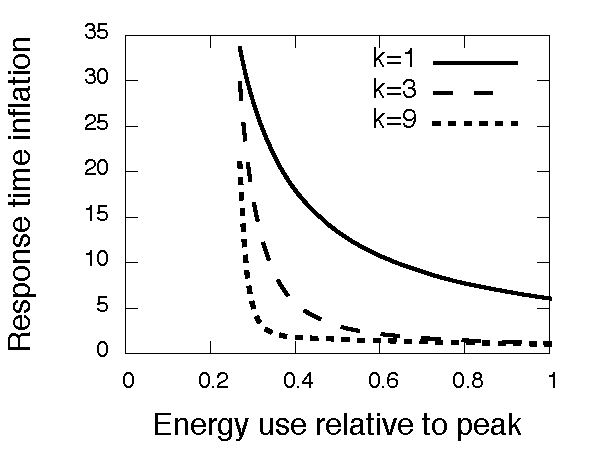
\includegraphics[scale=0.4]{graphs/vary-k.pdf}
%	\caption{}
%	\label{fig:vary-k}
%        \end{subfigure}
%\begin{subfigure}[b]{0.20\textwidth}
%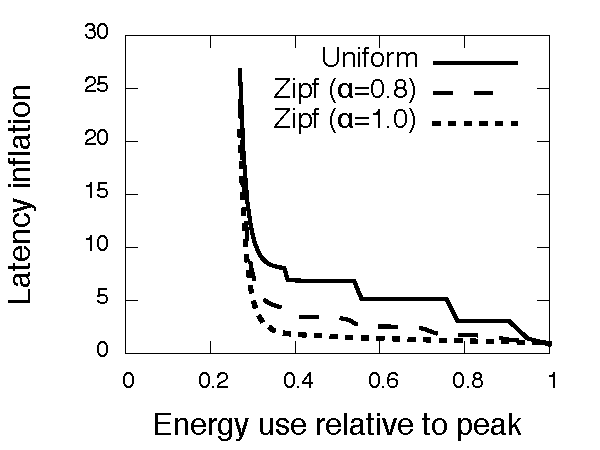
\includegraphics[scale=0.4]{graphs/vary-z.pdf}
%	\caption{}
%	\label{fig:vary-z}
%        \end{subfigure}
%\caption{Energy-latency tradeoff for (a) varying models of server latency for a Zipf workload ($\alpha$ = 1.0) and (b) workloads with varying Zipf exponents.}
%\end{figure}

\textbf{Numerical example:} We evaluate the evaluate the energy-latency tradeoff for Zipfian content popularity distributions. We assume that the server's utilization vs. latency profile is given by $f(u) = Cu^K$, $K>=1$ is a model parameter and $C$ is a constant latency. Other model parameters are as follows: each server has a capacity = 1 request/sec, total load $L$ = 15 requests/sec, latency from clients to servers $A$ = 10 ms, latency from servers to origin servers $B$ = 100 ms, server latency coefficient $C$ = 400 ms, idle power fraction $I$ = 0.5, total number of unit-sized content $M$ = 100 million, storage per server $S$ = 1 million, number of servers $N$ = 100. 

\begin{figure}[t]
\centering
    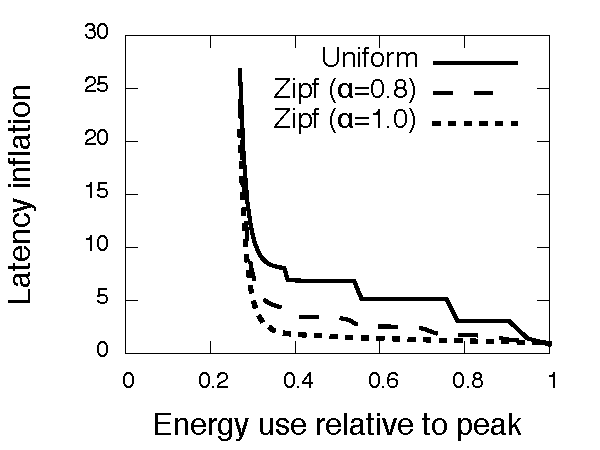
\includegraphics[scale=0.4]{graphs/vary-z.pdf}

  \caption{Energy-latency tradeoff for workloads with varying Zipf exponents.}
    \label{fig:vary-z}
\end{figure}

%\begin{figure}[t]
%\centering
%\begin{subfigure}[b]{0.23\textwidth}
%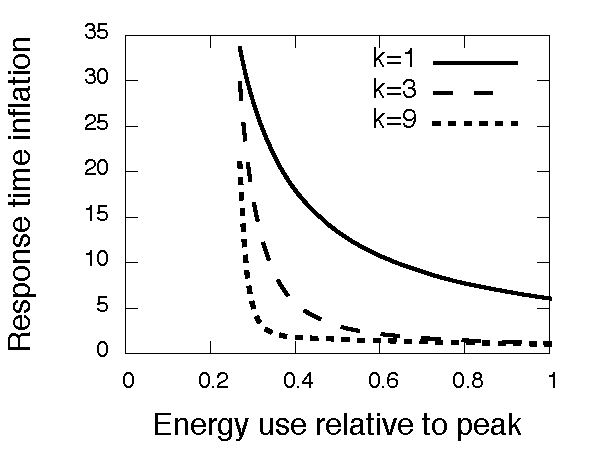
\includegraphics[scale=0.4]{graphs/vary-k.pdf}
%	\caption{}
%	\label{fig:vary-k}
%        \end{subfigure}
%\begin{subfigure}[b]{0.20\textwidth}
%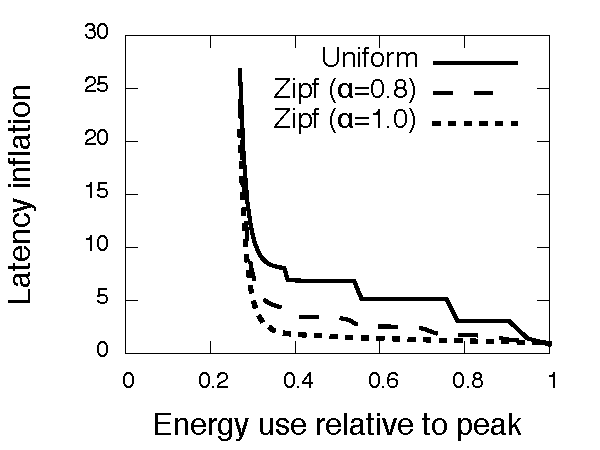
\includegraphics[scale=0.4]{graphs/vary-z.pdf}
%	\caption{}
%	\label{fig:vary-z}
%        \end{subfigure}
%\caption{Energy-latency tradeoff for (a) varying models of server latency for a Zipf workload ($\alpha$ = 1.0) and (b) workloads with varying Zipf exponents.}
%\end{figure}

%In Figure \ref{fig:vary-k} and Figure \ref{fig:vary-z}, the energy use is shown relative to the peak energy use with $N$ = 100 active servers, and latency inflation is shown relative to the least latency observed in each graph.		

%We assume that the server's utilization vs. latency profile $f(u) = Cu^K$, wherein $K>=1$ is a model parameter and $C$ is a constant latency. As $K$ increases from 1 to $\infty$, the latency profile becomes increasingly skewed. 

%In order to calculate the change in the hit rate when storage is reduced from $NS$ to $nS$, we use the following characteristic-time model \cite{che2002hierarchical}.
%\TBD{ [Equations here?]}
						
%Figure \ref{fig:vary-k} presents results for three models of server queuing latency with parameters $k$ = 1, 3 and 9; the Zipf exponent of the workload is $\alpha$ = 1.0 in all cases. In our model, the hit rates are independent of the server latency model. Therefore, the differences in latency among the curves is entirely due to a change in the server latency. We observe that the curve with $k$ = 9 achieves a significantly better energy-latency tradeoff than the curve k = 1. Further, the curve with $k$ = 9 stays nearly flat as energy use reduces by 60\% over peak. The reason is that server latencies remain a small fraction of latencies even at high utilization for $k$ = 9, and as a result, significant energy savings can be achieved with a small latency inflation.

Figure \ref{fig:vary-z} presents results for workloads with Zipf exponent $\alpha$ = 1.0, 0.8 and 0; $\alpha = 0$ results in a uniform distribution. The energy use is shown relative to the peak energy use with $N$ = 100 active servers, and latency inflation is shown relative to the least latency in the graph. The server  latency model parameter is $K$ = 9 for all workloads which implies that the difference in latencies among them is due to a difference in  miss rates. We observe that workloads with higher Zipf exponents achieve a better energy-latency tradeoff. The reason is that a higher Zipf exponent means that most of the hits result from a small fraction of objects, so reducing the available storage only results in a small increase in miss rates. 
%A key implication is that real workloads which commonly exhibit a Zipf exponent close to 1.0 \cite{fayazbakhsh2013less} can expect to achieve a good energy vs. latency tradeoff.
	

\textbf{Summary:}
Our simple expository model suggests that the energy vs. latency tradeoff is more favorable as the skew in the server's utilization vs. latency profile increases and the skew in the content popularity distribution increases. Admittedly, this simplistic model has several critical limitations as it (1) does not consider workload dynamics, (2) assumes a perfect load balance among servers, (3) ignores the overhead of coordination between servers, and (4) implicitly assumes that the utilization vs. latency behavior and the cache size vs. miss rate behavior can be approximated by treating the \cdc\ as a single logical server of the same total capacity, ignoring the network fabric entirely. 

Thus, a natural question is what do real, achievable energy vs. latency inflation tradeoffs look like in \cdc s? 
Further, does an increase server load or an increase in cache miss rates cause a greater impact on latency? 
To answer these questions, we present the design and implementation of Shrink and evaluate the tradeoff using a real workload from a large \cdc\  in the next two sections.